\documentclass[a4paper]{article}
\usepackage[utf8]{inputenc}
\usepackage[spanish, es-tabla, es-noshorthands]{babel}
\usepackage[table,xcdraw]{xcolor}
\usepackage[a4paper, footnotesep = 1cm, width=20cm, top=2.5cm, height=25cm, textwidth=18cm, textheight=25cm]{geometry}
%\geometry{showframe}

\usepackage{tikz}
\usepackage{amsmath}
\usepackage{amsfonts}
\usepackage{amssymb}
\usepackage{float}
\usepackage{graphicx}
\usepackage{caption}
\usepackage{subcaption}
\usepackage{multicol}
\usepackage{multirow}
\setlength{\doublerulesep}{\arrayrulewidth}
\usepackage{booktabs}

\usepackage{hyperref}
\hypersetup{
    colorlinks=true,
    linkcolor=blue,
    filecolor=magenta,      
    urlcolor=blue,
    citecolor=blue,    
}

\newcommand{\quotes}[1]{``#1''}
\usepackage{array}
\newcolumntype{C}[1]{>{\centering\let\newline\\\arraybackslash\hspace{0pt}}m{#1}}
\usepackage[american]{circuitikz}
\usetikzlibrary{calc}
\usepackage{fancyhdr}
\usepackage{units} 

\graphicspath{{../Calculos-Potencia/}{../Caracteristicas/}{../Consideraciones/}{../Gain-Stage/}{../Input-Stage/}{../Output-Stage/}{../Simulaciones/}{../Alimentacion/}{../Conclusiones/}}

\pagestyle{fancy}
\fancyhf{}
\lhead{22.12 Electrónica II}
\rhead{Mechoulam, Lambertucci, Rodriguez, Londero, Scala}
\rfoot{Página \thepage}

\begin{document}

\subsection{Introducción}

La etapa de entrada de un amplificador cumple con la función de restar a la entrada la señal proveniente de la realimentación, para así obtener la señal deseada de error, a partir de la cual se confecciona la salida del sistema.

\subsection{Distorsión}

La distorsión puede ser provocada o provenir de distintas fuentes. Los amplificadores que se valen del uso de pares diferenciales como entrada se caracterizan por poseer un bajo offset de continua, dado a la cancelación de los voltages de $V_{BE}$. Pero mucho más notorio e importante es que la corriente de mantenimiento no atraviesa la red de realimentación. Finalmente, una ventaja también a destacar es que posee una linealidad superior a las entradas basadas en un solo transistor. Se puede observar la comparación de distorsión entre una etapa diferencial frente a una individual en la Figura (\ref{fig:thd1}).

Es muy importante reflejar que esta etapa debe la que posee la mínima distorsión, por sobre las demás, ya que las señales que maneja son pequeñas, dándose el aumento de estas en la etapa de amplificación.    

%, trim = {0 0 0 20},clip
\begin{figure}[H]
\centering
	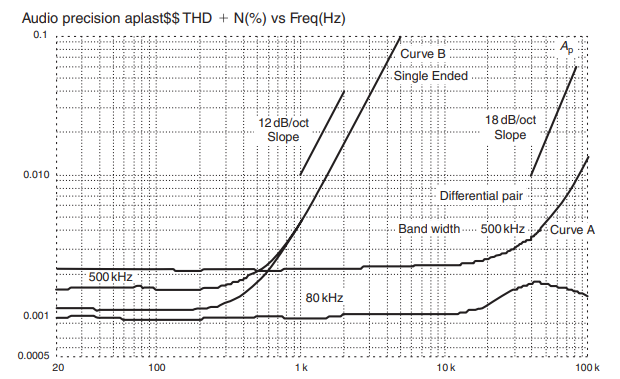
\includegraphics[width=0.8\textwidth]{ImagenesInput-Stage/thd1.PNG}
	\caption{Comparación de THD en función de la frecuencia.}
	\label{fig:thd1}
\end{figure}

Si bien, seleccionando adecuadamente las resistencias del circuito se puede balancear el par, quedan pendientes ciertos parámetros. Las corrientes de colectores deben ser lo más similares posibles. Debe existir una precisión del $1\%$ o mejor para poder optimizar la linealidad del la etapa, y de esta forma, reducir la distorsión en altas frecuencias.
\begin{figure}[H]
\centering
	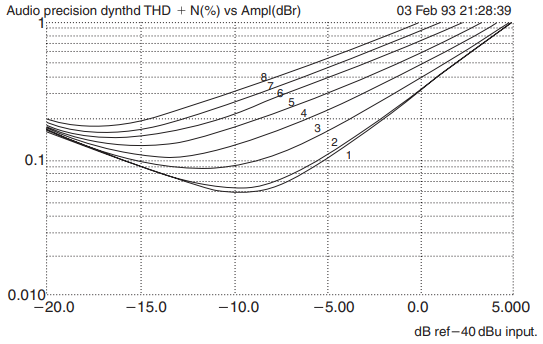
\includegraphics[width=0.8\textwidth]{ImagenesInput-Stage/thd2.PNG}
	\caption{THD en función de la amplitud al variar el balance de la corriente del colector. Número de curva y distorsión especificadas en la Tabla (\ref{tab:thd2}).}
	\label{fig:thd2}
\end{figure}

\begin{table}[H]
\centering
\begin{tabular}{cc}
\hline
\textbf{Número de curva} & \textbf{Variación $\mathbf{I_C}$ [\%]} \\ \hline
1                        & 0                    \\
2                        & 0.5                  \\
3                        & 2.2                  \\
4                        & 3.6                  \\
5                        & 5.4                  \\
6                        & 6.9                  \\
7                        & 8.5                  \\
8                        & 10             		\\
\hline
\end{tabular}
\caption{Número de curva y distorsión de la Figura (\ref{fig:thd2}).}
\label{tab:thd2}
\end{table}

Una opción valida (e implementada en este diseño) se basa en el uso de resistencias en los emisores para ajustar dicho parámetro. Es importante recordar que dichos elementos no deben ser lo suficientemente grandes como para que afecte el ruido térmico.

\subsection{Linealidad y corriente de colector}

La transconductancia aumenta con la corriente de colector. Elevar este último parámetro es posible y relativamente sencillo. Una técnica empleada para poder mejorar la linealidad en altas frecuencias consiste en aumentar la corriente mencionada para luego reducirla a través del lazo de realimentación negativa. Esta no linealidad es atribuida a la resistencia del $R_E$ del emisor, la cual no es una resistencia física, sino que una resultante de la expresión de la pendiente de la corriente de colector. 

La corriente de mantenimiento a la entrada es uno de los parámetros que define el máximo slew rate (SR). Otro factor importante que lo limita es el polo dominante proveniente del capacitor de Miller. Este último es solucionado por los requerimientos que se deben cumplir para conseguir la estabilidad. Por otro lado, aumentar la corriente de colector puede aumentar el factor de SR sin afectar la estabilidad, siempre y cuando, la transconductancia se mantenga en el valor deseado. 

A pesar de ello, existen límites para esta corriente. El aumento de las corrietnes de bias, como la caida de tensión a través de las resistencias son algunos ejemplos. El factor más limitante es la potencia disipada a lo largo de esta etapa, ya que no siempre deja margen para incrementar la $I_C$. 


\textbf{buffer a la salida del par diferencial para que las resistencias del amp dif sean más pequeñas}

\textbf{ganancia baja}

\end{document}